\chapter{Coordination Mechanism of Communication and Computation}\label{sec:iv}

\section{Introduction}\label{sec:iv-introduction}

Recent scientific research has been taking major advantage of
computational analysis and simulation. Sustained growth in the volume of
data generated by scientific experiments has lead to a rise in the
importance of data-intensive computing. For example, approximately 15PB
of experimental data is annually generated and processed at the Large
Hadron Collider (LHC), an experimental facility for high energy
physics~\autocite{Bird2011}.

Today, in general, data-intensive computations are performed on
high-performance computer clusters. A computer cluster is composed of a
set of computing nodes connected to a high-performance network, usually
referred to as an \emph{interconnect}. Applications designed to run on
computer clusters are based on a parallel distributed processing model.
In this processing model, a large computation is decomposed into smaller
fractions of computation and is then performed by processes running in
parallel. These processes communicate with each other for data exchange
and synchronization. For this reason, the inter-node communication
performance among processes can significantly impact the total
performance of data-intensive applications. Recent advancements of high
performance computing has heavily relied upon the high degree of
parallelism rather than the improvement of CPU clock speed.
Consequently, the total number of processes and computing nodes involved
in a computation has kept increasing. As a result, communication between
distributed processes is becoming the principal bottleneck of
data-intensive applications.

Each application running on a computer cluster has a distinct pattern of
communication among processes~\autocite{Kamil2010}. These communication
patterns are difficult to predict precisely in prior to the execution of
the application. Furthermore, most of the current interconnects
available have adopted static network control and thus are unable to
adaptively reconfigure themselves to match requirements from
applications. In fact, in InfiniBand~\autocite{Buyya2009}, which is
a currently dominant interconnect technology, the forwarding tables on
switches are usually pre-configured and remain unchanged until hardware
failure or topology change occurs.

Furthermore, current interconnects are designed to be over-provisioned
in order to satisfy the communication performance requirements of
various applications with diverse communication patterns. Such
over-provisioned interconnects are designed and provided with sufficient
network resources (\emph{e.g.} bandwidth) to minimize the overload of
interconnect such as congestion.

However, recent scale-out in the number of computing nodes has revealed
two potential shortcomings of over-provisioned designs. First, the cost
of building interconnects has become increasingly higher, which makes it
difficult to implement over-provisioned designs. This increased cost is
because of the scale and complexity of interconnects that grow
superlinearly as the number of computing nodes increases. The second
shortcoming is the underutilization of interconnects. A discrepancy
between the performance characteristics of the over-provisioned
interconnect and the aggregated network requirements of the applications
may cause some portion of the interconnect not being fully utilized.

Based on these considerations, we believe that a novel cluster
architecture which dynamically controls the packet flow in the
interconnect based on the communication pattern of the application can
alleviate the aforementioned two shortcomings of conventional
over-provisioned designs. For this reason, Software-Defined Networking
enhanced Message Passing Interface (\emph{SDN-enhanced MPI}), which is
an unconventional MPI framework that incorporates flexible network
controllability of SDN into interconnects, was proposed in our past
research. Furthermore, in past research towards SDN-enhanced MPI, we
have demonstrated that the acceleration of collective MPI communication
is feasible.

However, a technical challenge still remained in this research; namely,
applying our research achievements to real-world MPI applications. In
the preliminary stage of our current research so far, we focused on
verifying the feasibility of our idea by investigating whether
individual MPI collective communications could be accelerated or not.
Therefore, how MPI communication accelerated with SDN could be
synchronized with the execution of an MPI application remained a
question that required a new technical innovation.

To this end, we propose \emph{UnisonFlow}, a mechanism for SDN-enhanced
MPI to perform network control in synchronization with the execution of
an MPI application, based on the strategy shown
in~\autocite{Takahashi2015}. The synchronization does not incur a large
overhead so it avoids performance degradation of the applications.
Furthermore, the proposed mechanism is designed to work on actual
hardware OpenFlow switches, and is not limited to software switches or
specialized hardware.

The main contributions of this chapter are summarized as follows:

\begin{itemize}
\item
  UnisonFlow, a software-defined coordination mechanism of network
  control and execution of an MPI application is proposed.
\item
  A low-overhead implementation of the proposed concept that works on
  actual hardware OpenFlow switches is presented.
\item
  An experiment is carried out to verify whether the interconnect
  control is successfully performed in synchronization with the
  execution of an application.
\item
  A performance measurement of point-to-point communication is conducted
  to evaluate the overhead incurred by the proposed mechanism.
\end{itemize}

The remainder of this chapter is organized as follows.
Section~\ref{sec:iv-objective} introduces SDN-enhanced MPI and its key
technologies. Subsequently, the challenge to realize SDN-enhanced MPI is
derived. Section~\ref{sec:iv-proposal} describes our proposed mechanism and its
implementation. Section~\ref{sec:iv-evaluation} shows the result of the experiments
conducted to demonstrate the feasibility of the proposal.
Section~\ref{sec:iv-related-work} reviews related literature and clarifies the
contributions of this chapter. Finally, Section~\ref{sec:iv-conclusion} discusses
future issues to be tackled and concludes this chapter.

\section{Research Objective}\label{sec:iv-objective}

This section first briefly describes the two key technologies of
SDN-enhanced MPI:\@ the Message Passing Interface (MPI) and Software
Defined Networking (SDN). After outlining the current development status
of SDN-enhanced MPI, the central challenge in realizing a practical
SDN-enhanced MPI is clarified.

\subsection{SDN-enhanced MPI}\label{sec:iv-sdn-mpi}

The basic idea of SDN-enhanced MPI is to incorporate the flexible
network controllability of SDN into MPI\@. As described in
Section~\ref{sec:i-mpi}, MPI mainly focuses on hiding the
complexity of the underlying network architecture. Therefore, MPI does not
provide any functionality for explicitly controlling the network. Integrating
SDN into MPI could complement such lack of a network control feature in MPI
and allow MPI to optimize the packet flow in the network in accordance with
the communication pattern of applications.

At the time of writing this paper, we have applied the above described
basic idea to two collective MPI primitives, MPI\_Bcast and
MPI\_Allreduce as proof of concept. Experiments conducted on a real
computer cluster comprising bare metal servers and hardware OpenFlow
switches have demonstrated that the execution time of these primitives
has been successfully reduced~\autocites{Dashdavaa2013}{Takahashi2014}.
SDN-enhanced MPI\_Bcast~\autocite{Dashdavaa2013} accelerates MPI\_Bcast
by utilizing the hardware multicast functionality of OpenFlow switches.
SDN-enhanced MPI\_Allreduce~\autocite{Takahashi2014} dynamically
reconfigures the path allocation based on the communication pattern of
MPI\_Allreduce so that congestion in links is minimized.

\subsection{Central Challenge of SDN-enhanced MPI}

The central challenge in realizing a practical SDN-enhanced MPI lies in
a coordination mechanism between the application and network control.
Although the previous works on SDN-enhanced MPI have shown the
feasibility of accelerating individual primitives as described in
Section~\ref{sec:iv-sdn-mpi}, actual MPI applications have not yet
taken advantage of network programmability brought by SDN, since each of
the distinct network control algorithms designed for an MPI primitive
cannot be activated along with the execution of an MPI application. In
other words, no mechanism exists that conveys the type and option of the
MPI primitive being executed at the moment by an application to the
network controller in charge of acceleration of the corresponding
primitive.

In this chapter, we realize a software-defined coordination mechanism to
perform network control in synchronization with the execution of an
application. Furthermore, the following technical requirements must be
met by the mechanism:

\begin{itemize}
\item
  \emph{Low overhead}: The overhead incurred by the proposed coordination
  mechanism should not degrade the communication performance of MPI, since the
  final goal is to improve the total performance of the MPI application.
\item
  \emph{Interoperability with hardware OpenFlow switches}: We place emphasis
  on developing a practical implementation that works on computer clusters.
  Therefore, the mechanism should work on actual hardware OpenFlow switches,
  and should not be limited to software switches or specialized hardware.
\item
  \emph{Compatibility with existing MPI library}: To mitigate the
  cost to port existent MPI applications on SDN-enhanced MPI, the existent MPI
  application should work on SDN-enhanced MPI without the source code being
  modified or recompiled. Compatibility with existing MPI implementations is
  essential for the portability of applications.
\end{itemize}

\section{Proposal}\label{sec:iv-proposal}

\subsection{Basic Idea}\label{sec:iv-basic-idea}

The basic idea of UnisonFlow is to embed MPI context information as a
\emph{tag} into each packet released through the MPI library and handle
packets based on their tags in switches. The tag is stored in the header
field of each packet. In this paper, MPI context information is defined
as a collection of application-aware data which identifies an
communication of an MPI communication primitive. Specifically, an MPI
primitive type, source/destination rank and communicator constitute MPI
context information.

A straightforward approach to realize application-aware network control
is to enhance the packet processing feature of OpenFlow switches in a
way that switches can read application-layer information from packets
and then make decisions based on that information. However, this
approach requires significant alteration to the switch hardware itself
and the OpenFlow protocol, because packet processing on switches is
mostly performed on fixed dedicated hardware components. The proposed
mechanism stores application-layer information into a header field of
packets so that OpenFlow switches can perform application-aware packet
flow control.

In detail, the tag is embedded into the destination MAC address field of
the packet header field. The location of the destination MAC address
field in a packet and the binary layout of a tag are shown in
Fig.~\ref{fig:binary-layout}.

\begin{figure}
    \centering
    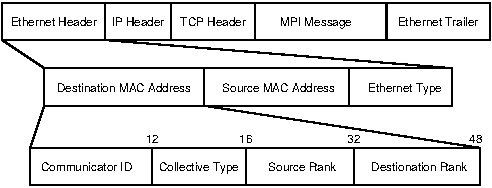
\includegraphics[width=0.8\linewidth]{binary-layout}
    \caption{Tag Information Embedded in a Packet}%
    \label{fig:binary-layout}
\end{figure}

Two main reasons exist for using the destination MAC address header
field. The first reason is that the MAC address is defined as one of the
header fields that can be used as a matching condition in OpenFlow. For
this reason, there is no need to extend or modify existing OpenFlow
switches to support this header field. The second reason is explained
from the advantage in the number of installable flow entries. Although
there are header fields other than the destination MAC address that can
be used as a matching condition in OpenFlow, switches are typically
equipped with a special hardware dedicated for L2 header field lookups.
As a result, more flow entries that include only L2 header fields can be
stored than the flow entries with other header fields.

\subsection{Architecture}

\subsubsection{Overview}

Figure~\ref{fig:overall-arch} illustrates an overview of UnisonFlow. At
this stage of research, it is assumed that a computer cluster executes a
single MPI application because our research target is the acceleration
of inter-node communication in MPI\@. The operating system of computing
nodes is assumed to be Linux.

\begin{figure}
    \centering
    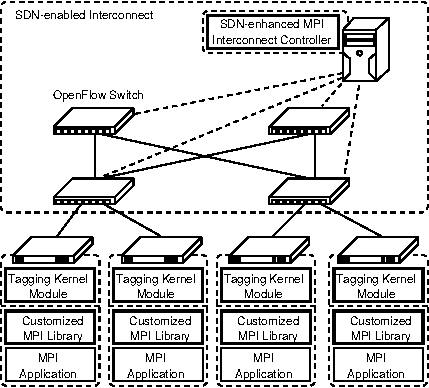
\includegraphics[width=0.7\linewidth]{overall-arch}
    \caption{Overall Architecture of UnisonFlow}%
    \label{fig:overall-arch}
\end{figure}

We have developed three major software modules that constitute this
architecture (bold rectangles in Fig.~\ref{fig:overall-arch}). The first
module is the \emph{Interconnect Controller}, which is basically an
OpenFlow controller responsible for installing flow entries into
OpenFlow switches. The interconnect controller was developed based on
the Ryu SDN controller framework~\autocite{Ryu2014}. The second module
is the \emph{Tagging Kernel Module}. It resides in the kernel space of
each computing node. The role of the tagging kernel module is to extract
MPI context information from each packet emitted by the MPI library,
encode this context information as a tag and then apply it to the
packet. The third module is the \emph{Customized MPI Library,} which is
dynamically linked to the MPI application. MPICH~\autocite{Gropp2002},
an implementation of MPI, was extended so that it meets our needs.
Specifically, it was enhanced to communicate with the tagging kernel
module and to send active connection information to the kernel module.

\subsubsection{Intra-node architecture}

On each computing node, the tagging kernel module and MPI library work
together to embed MPI context information as a tag into each packet. The
kernel module performs the actual tagging procedure, whereas the MPI
library provides the kernel module with supplementary information used
for filtering out non-MPI traffic.

As described in Section~\ref{sec:iv-basic-idea}, UnisonFlow exploits the
destination MAC address field of a packet as a place to store the
corresponding tag. To implement this, a functional component that
dynamically rewrites MAC address fields of packets is essential.

As a possible solution for the functional component on the Linux kernel,
we have considered \emph{ebtables}, \emph{raw socket} and \emph{protocol
handler}~\autocite{Rosen2013}. Ebtables is a widely adopted L2 packet filter
implemented on top of the netfilter framework. It mainly features L2 packet
filtering and Network Address Translation~(NAT). Raw sockets are special type
of sockets that give user space programs access to the whole packet including
protocol headers. TCP/UDP sockets only allows users space programs to read or
write TCP/UDP payloads, whereas raw sockets allows programs to read and write
TCP/UDP, IP and Ethernet protocol headers. In return, the user space program
has the full responsibility to handle the network protocol correctly. The
network stack of Linux kernel is designed to be extensible so that new network
protocols can be added relatively easily. New protocols can be implemented
as a protocol handler, which is essentially a call back function that is
invoked when a packet is sent or received. When implemented in a loadable
kernel module, protocol handlers can be added without recompiling the kernel.

Out of these potential solutions,
we have adopted the protocol handler because it achieves both
flexibility in rewriting of the packets depending on their payload and
minimal alteration to the MPI library. As previously described, ebtables
has a MAC NAT feature; however, it has a limitation where the MAC
addresses can only be translated to pre-configured addresses. On the
other hand, the use of a raw socket results in an extensive modification
of the MPI library, since it requires the MPI library to handle the
TCP/IP stack. In contrast to these two methods, the use of the protocol
handler facilitates the interception of packets in the network stack of
the kernel and arbitrary modifications to those packets. For this
reason, we can utilize the network stack of the kernel and avoid
re-implementing another network stack. Moreover, the whole packet
including header and payload can be read and written by the protocol
handler for dynamically rewriting the MAC address fields of packets.

Figure~\ref{fig:intra-node-flow} illustrates how MPI packets are
processed on a computing node. The solid arrows represent packet flows
generated by an MPI application. The dashed arrow represents interaction
between software modules.

\begin{figure}
    \centering
    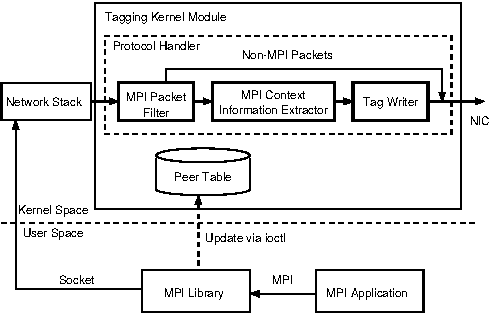
\includegraphics[width=0.8\linewidth]{intra-node-flow}
    \caption{Intra-node Packet Flow}%
    \label{fig:intra-node-flow}
\end{figure}

Once the tagging kernel module is loaded into the kernel space at the
boot time of the Linux operating system, the kernel module registers its
own protocol handler to the kernel using the
\lstinline!dev_add_pack! API\@. This protocol handler is
called every time a packet is sent out from the network stack to the
Network Interface Card (NIC). Intercepted packets sequentially undergo
three major phases of packet processing, which are performed by the
following three components (bold rectangles in
Fig.~\ref{fig:intra-node-flow}), respectively:

\begin{enumerate}
\def\labelenumi{\arabic{enumi}.}
\item
  \emph{MPI packet filter}: Packets generated by SSH, remote file
  systems, and any programs other than MPI are immediately forwarded to
  the NIC\@. To investigate whether a packet originates from MPI or not,
  this component looks up the \emph{peer table} maintained by the
  tagging kernel module and verifies if the packet is a part of the TCP
  connections opened by the MPI library. The peer table is designed as a
  hash table of all TCP connections to other processes opened by MPI\@.
  The 4-tuple (source IP, destination IP, source port and destination
  port) of each packet is used to identify a TCP connection.
\item
  \emph{MPI context information extractor}: This component extracts the
  MPI context information from packets by reading and parsing their
  message envelope. The message envelope is essentially a header that is
  prepended to every MPI message by the MPI library for identification.
  Although the message envelope is prescribed in the MPI
  specification~\autocite{MessagePassingInterfaceForum2015}, its actual binary
  layout is implementation dependent.
\item
  \emph{Tag writer}: This component encodes the context information
  extracted in the previous phase as a virtual MAC address and writes it
  into the packet. The virtual MAC address is generated by packing the
  components of MPI context information into the binary format shown in
  Fig.~\ref{fig:binary-layout}. Technically, the MAC addresses of
  packets can be modified by simply overwriting the specific position of
  the \lstinline!sk_buff! structure, which is the
  internal representation of network packets in the kernel.
\end{enumerate}

As described, the tagging kernel module maintains the peer table to keep
track of all connections opened by the locally-running MPI process to
other MPI processes running on remote computing nodes. In order to
update the content of the peer table in accordance with the internal
information of the MPI library, the MPI library has been enhanced to
provide this information to the kernel module. As the communication
channel between the MPI library and kernel module, the
\lstinline!ioctl! system call has been leveraged. These
modifications have been made so that functional compatibility with the
original MPI library was guaranteed.

\subsubsection{Inter-node architecture}

Switches composing the interconnect forward packets based on their tag
value. These forwarding rules are stored in the form of flow entries and
managed by the centralized interconnect controller.

The decision about how a packet is forwarded is made by the \emph{MPI
primitive module}, which is a pluggable software component integrated
into the interconnect controller. A unified interface between the MPI
primitive module and the interconnect controller is defined for
simplified development and integration of primitive modules. Each MPI
primitive module is expected to be designed dedicatedly for a single
type of MPI primitive.

Figure~\ref{fig:inter-node-flow} illustrates an example of the packet
flow between two remote computing nodes. When the interconnect
controller receives a packet-in message caused by an unmatched packet
(step 1 in Fig.~\ref{fig:inter-node-flow}), the controller decodes the
tag embedded in the packet and extracts the MPI context information
(step 2). After that, the responsible MPI primitive module is invoked
with the context information as its input (step 3). The MPI primitive
module determines how a set of packets carrying the same context
information should be treated. Based on this decision, flow entries are
generated and then installed to relevant switches (step 4).

\begin{figure}
    \centering
    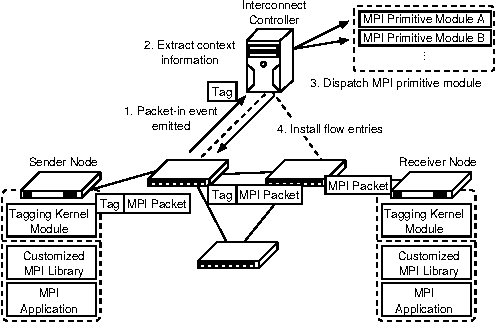
\includegraphics[width=0.8\linewidth]{inter-node-flow}
    \caption{Inter-node Packet Flow}%
    \label{fig:inter-node-flow}
\end{figure}

Note that NICs drop incoming packets whose destination addresses are not
the address of NICs unless they are put into promiscuous mode.
Therefore, the destination MAC address of tagged packets needs to be
restored to the true MAC address of its receiver node. This restoration
is achieved by appending an action for changing the MAC address field to
the flow entry installed on the switch adjacent to the receiver node.

\section{Evaluation}\label{sec:iv-evaluation}

Two experiments were conducted to examine the feasibility of UnisonFlow.
In the first experiment, the control of the interconnect is investigated
in terms of whether it is properly synchronized with the execution of
the application. In the second experiment, the overhead imposed by
UnisonFlow is evaluated.

\subsection{Experimental environment}

Both of the two experiments were conducted on the SDN-enabled computer
cluster shown in Fig.~\ref{fig:cluster-topology}. For the topology of
the interconnect, a two-tier fat-tree composed of six switches was
adopted because fat-trees are one of the most widely used topologies for
today's cluster systems. Note that each of the two physical switches was
divided to three logical switches due to a limited number of available
OpenFlow switches in our institution. In the following discussion, we
refer to the two upper layer switches as spine1 and spine2, whereas the
four lower layer switches are referred to as leaf1, leaf2, leaf3 and
leaf4, respectively. Spine switches and leaf switches were connected on
4 Gbps links, each of which was an aggregated link of four GbE links.
Six computing nodes were connected to a leaf switch; that is, 24
computing nodes in total. These computing nodes are hereinafter referred
to as node01 to node24. Leaf switches and computing nodes were
interconnected with 1Gbps Ethernet. A management node accommodating the
interconnect controller was also prepared.

\begin{figure}
    \centering
    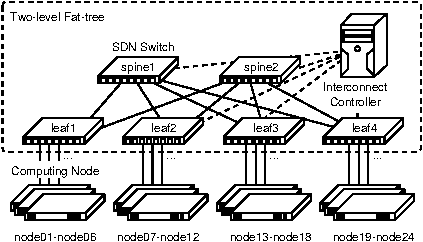
\includegraphics[width=0.8\linewidth]{cluster-topology}
    \caption{Overview of the Experimental Environment}%
    \label{fig:cluster-topology}
\end{figure}

For SDN switches, NEC ProgrammableFlow PF5240 has been adopted. The computing
node was a SGI Rackable Half-Depth Server C1001 equipped with the hardware and
software as shown in Table~\ref{tbl:node-spec}.

\begin{table}
    \centering
    \caption{Computing Node Specifications}%
    \label{tbl:node-spec}
    \begin{tabular}{ll}
        \toprule
        Name        & Spec                                        \\ \midrule
        CPU         & Intel Xeon E5-2620 2.00GHz 6core $\times$ 2 \\
        Memory      & 64GB (DDR3-1600 8GB $\times$ 8)             \\
        Network     & Gigabit Ethernet                            \\
        OS          & CentOS 7.2                                  \\
        Kernel      & Linux 3.10                                  \\
        MPI Library & MPICH 3.1.4                                 \\ \bottomrule
    \end{tabular}
\end{table}

\subsection{Verification of coordination mechanism}

The first experiment was conducted to verify whether the dynamic control
of packet flows on the interconnect was performed in synchronization
with the execution of the application. To verify the synchronization
between interconnect control and execution of the application, an MPI
application which sequentially executes two different MPI primitives has
been developed. The interconnect controller applies different routing
strategies for each primitive as MPI primitive modules. We then observe
the packet flow on the interconnect using the port counters of switches
to verify if the interconnect control can successfully switch from one
to another when the MPI primitive executed changes.

The detailed experimental setup is as follows. The MPI application
executes an iteration of MPI\_Bcast followed by another iteration of
MPI\_Reduce. List~\ref{lst:sync-mpi-app} shows a simplified source code
of this application. The process with rank 0 is specified as the root
process for both MPI\_Bcast and MPI\_Reduce. The rank 0 process is
configured to run on node01, which is connected to switch leaf1.
Furthermore, the MPI application records the time where each of the
following three events occurs: the start of the MPI\_Bcast iteration
(\(t_1\)), the start of the MPI\_Reduce iteration (\(t_2\)) and the
finish of the MPI\_Reduce iteration (\(t_3\)). This timing information
is used to investigate the relationship between the execution of the MPI
application and the traffic change in the interconnect.

\begin{figure}
    \centering
    \begin{subfigure}{.45\linewidth}
        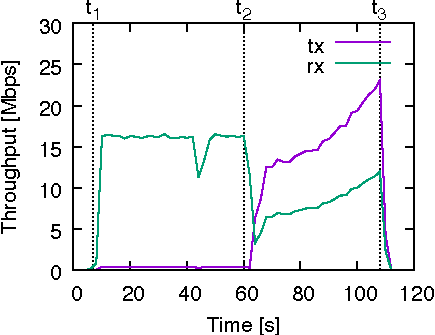
\includegraphics[width=.95\linewidth]{coll-conv-1-2560}
        \caption{At Port 0xa00 (spine1) \newline Towards Port 0xa00 (leaf1)}%
        \label{fig:spine1-leaf1-conv}
    \end{subfigure}
    \begin{subfigure}{.45\linewidth}
        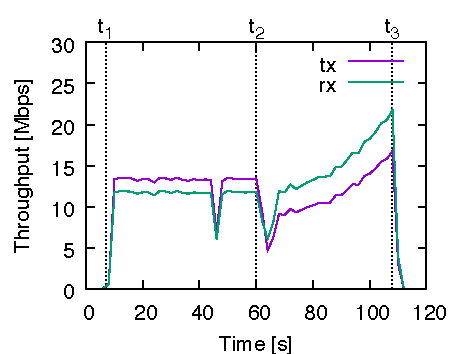
\includegraphics[width=.95\linewidth]{coll-conv-1-2816}
        \caption{At Port 0xb00 (spine1) \newline Towards Port 0xa00 (leaf2)}%
        \label{fig:spine1-leaf2-conv}
    \end{subfigure}
    \begin{subfigure}{.45\linewidth}
        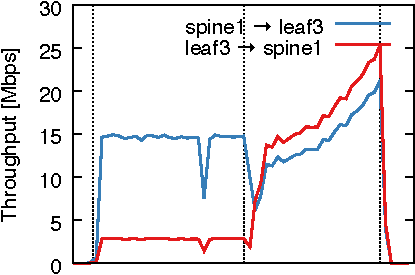
\includegraphics[width=.95\linewidth]{coll-conv-1-3072}
        \caption{At Port 0xc00 (spine1) \newline Towards Port 0xa00 (leaf3)}%
        \label{fig:spine1-leaf3-conv}
    \end{subfigure}
    \begin{subfigure}{.45\linewidth}
        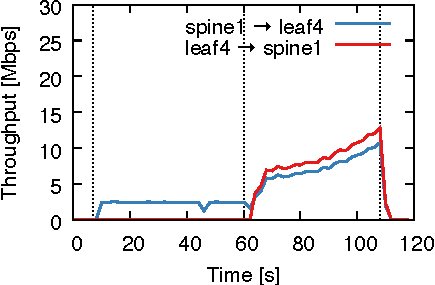
\includegraphics[width=.95\linewidth]{coll-conv-1-3328}
        \caption{At Port 0xd00 (spine1) \newline Towards Port 0xa00 (leaf4)}%
        \label{fig:spine1-leaf4-conv}
    \end{subfigure}
    \caption{Throughput Measured at Ports on Switch spine1 (conventional)}%
    \label{fig:coll-spine1-conv}
\end{figure}

\begin{figure}
    \begin{subfigure}{.45\linewidth}
        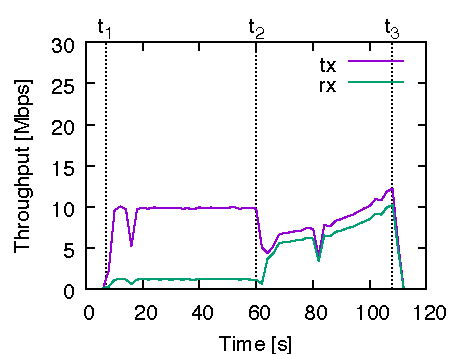
\includegraphics[width=.95\linewidth]{coll-conv-2-2560}
        \caption{At Port 0xa00 (spine2) \newline Towards Port 0xa00 (leaf1)}%
        \label{fig:spine2-leaf1-conv}
    \end{subfigure}
    \begin{subfigure}{.45\linewidth}
        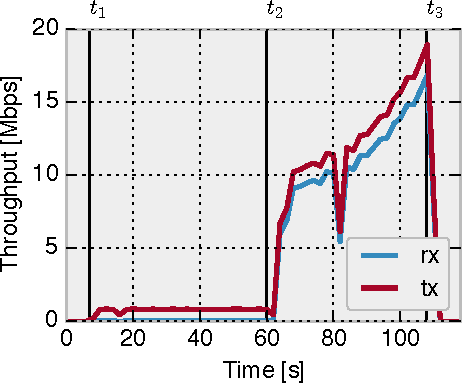
\includegraphics[width=.95\linewidth]{coll-conv-2-2816}
        \caption{At Port 0xb00 (spine2) \newline Towards Port 0xa00 (leaf2)}%
        \label{fig:spine2-leaf2-conv}
    \end{subfigure}
    \begin{subfigure}{.45\linewidth}
        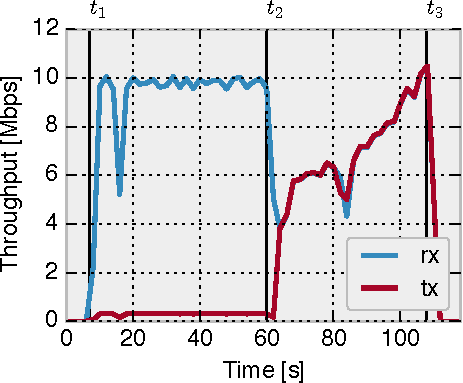
\includegraphics[width=.95\linewidth]{coll-conv-2-3072}
        \caption{At Port 0xc00 (spine2) \newline Towards Port 0xa00 (leaf3)}%
        \label{fig:spine2-leaf3-conv}
    \end{subfigure}
    \begin{subfigure}{.45\linewidth}
        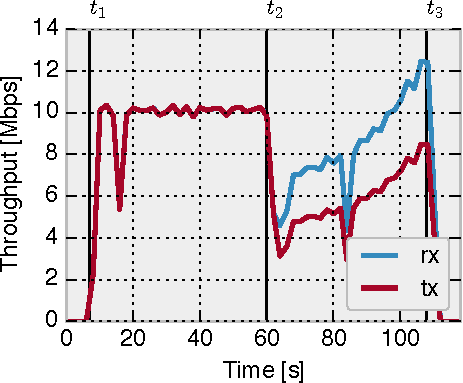
\includegraphics[width=.95\linewidth]{coll-conv-2-3328}
        \caption{At Port 0xd00 (spine2) \newline Towards Port 0xa00 (leaf4)}%
        \label{fig:spine2-leaf4-conv}
    \end{subfigure}
    \caption{Throughput Measured at Ports on Switch spine2 (conventional)}%
    \label{fig:coll-spine2-conv}
\end{figure}

Each MPI primitive is repetitively executed because a single invocation
of these primitives completes too quickly to observe the traffic change.
The port counters of PF5240 are updated approximately once a second.
This implies that instant traffic changes happening in less than one
second cannot be precisely observed. Since a single invocation of
MPI\_Bcast or MPI\_Reduce finishes in the order of milliseconds, we
repeat each primitive to make its total execution time longer so that we
can observe the traffic change using port counters.

\begin{lstlisting}[caption={Source code of MPI application}, label=lst:sync-mpi-app, float=htbp]
#include <mpi.h>
#define BUF_SIZE     (1000)
#define REPEAT_COUNT (10000)

char send_buf[BUF_SIZE];
char recv_buf[BUF_SIZE];

int main(int argc , char** argv) {
    MPI_Init(&argc , &argv);

    /* Record current time as $t_1$ */

    /* MPI_Bcast */
    for (i = 0; i < REPEAT_COUNT; i++) {
        MPI_Bcast(send_buf, BUF_SIZE, MPI_CHAR, 0,
                  MPI_COMM_WORLD);
    }

    /* Record current time as $t_2$ */

    /* MPI_Reduce */
    for (i = 0; i < REPEAT_COUNT; i++) {
        MPI_Reduce(send_buf, recv_buf, BUF_SIZE,
                   MPI_CHAR, MPI_SUM, 0,
                   MPI_COMM_WORLD);
    }

    /* Record current time as $t_3$ */

    MPI_Finalize();
}
\end{lstlisting}

Under the interconnect topology of this experimental environment, there
are always two possible paths between any two different leaf switches.
One is the path that contains spine1 (\emph{e.g.} leaf1 - spine1 -
leaf2) and the other path contains spine2 (\emph{e.g.} leaf1 - spine2 -
leaf2). The interconnect controller was deployed with a routing strategy
that assigns paths utilizing spine1 to the traffic generated by
MPI\_Bcast. In contrast, the traffic generated by MPI\_Reduce was set so
that it goes through spine2. Note that spine switches are never utilized
by traffic between two computing nodes under an identical leaf switch.
As a representative implementation of conventional networking
architecture, an SDN controller was employed with a Equal Cost Multi
Path (ECMP) routing strategy. To observe the traffic change in the
interconnect, a measurement module that periodically (every two seconds)
gathers and reports transmitted and received bytes of every switch port
was integrated into the interconnect controller. Based on these port
counter values, we calculated the throughput of the transmitted traffic
and the received traffic of each port.

Figures~\ref{fig:coll-spine1-conv} and \ref{fig:coll-spine2-conv} show
the change of throughput observed at the ports of switches spine1 and
spine2 when using ECMP\@. Both spine1 and spine2 were utilized during the
execution of MPI\_Bcast and MPI\_Reduce as a result of load balancing.
However, there is some inequality in the utilization of two spine
switches. This inequality is because ECMP distributes the traffic
workload not on the basis of not packets, but on flows.

MPICH, which is the MPI implementation used in UnisonFlow, has optimized
implementations for collective communications like other MPI libraries.
In particular, under the environment of this experiment, MPI\_Bcast uses
binomial tree algorithm while MPI\_Reduce uses the Rabenseifner's reduce
algorithm~\autocite{Rabenseifner2004}. As a result, MPI\_Bcast is not a
simple repeated point-to-point communication from the root process to
other processes, but involves communication between non-root processes.
For instance, Fig.~\ref{fig:spine1-leaf1-conv} indicates how the traffic
between spine1 and leaf1 changes. In detail, TX shows the outgoing
traffic from spine1 to leaf1, which is the aggregated traffic from the
computing nodes under leaf2, leaf3 and leaf4 to the computing nodes
under leaf1. In contrast, RX shows the aggregated traffic from computing
nodes under leaf1 to other computing nodes under leaf2, leaf3 and leaf4.

\begin{figure}
    \centering
    \begin{subfigure}{.45\linewidth}
        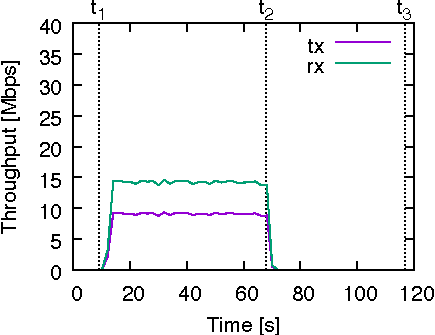
\includegraphics[width=.95\linewidth]{coll-prop-1-2560}
        \caption{At Port 0xa00 (spine1) \newline Towards Port 0xa00 (leaf1)}%
        \label{fig:spine1-leaf1-prop}
    \end{subfigure}
    \begin{subfigure}{.45\linewidth}
        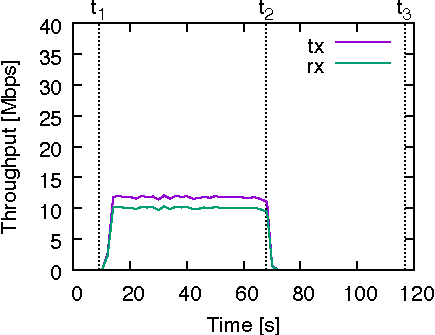
\includegraphics[width=.95\linewidth]{coll-prop-1-2816}
        \caption{At Port 0xb00 (spine1) \newline Towards Port 0xa00 (leaf2)}%
        \label{fig:spine1-leaf2-prop}
    \end{subfigure}
    \begin{subfigure}{.45\linewidth}
        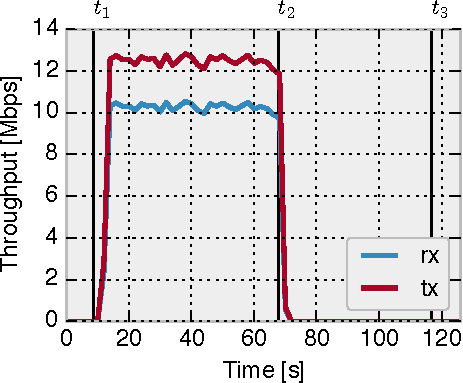
\includegraphics[width=.95\linewidth]{coll-prop-1-3072}
        \caption{At Port 0xc00 (spine1) \newline Towards Port 0xa00 (leaf3)}%
        \label{fig:spine1-leaf3-prop}
    \end{subfigure}
    \begin{subfigure}{.45\linewidth}
        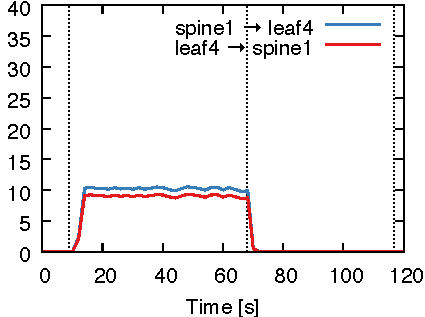
\includegraphics[width=.95\linewidth]{coll-prop-1-3328}
        \caption{At Port 0xd00 (spine1) \newline Towards Port 0xa00 (leaf4)}%
        \label{fig:spine1-leaf4-prop}
    \end{subfigure}
    \caption{Throughput Measured at Ports on Switch spine1 (proposed)}%
    \label{fig:coll-spine1-prop}
\end{figure}

\begin{figure}
    \begin{subfigure}{.45\linewidth}
        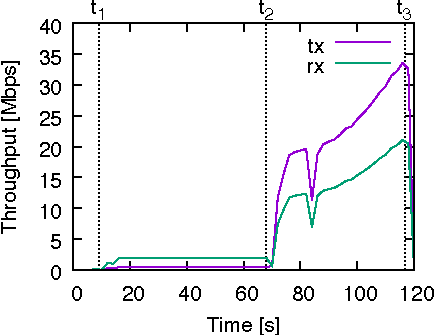
\includegraphics[width=.95\linewidth]{coll-prop-2-2560}
        \caption{At Port 0xa00 (spine2) \newline towards Port 0xa00 (leaf1)}%
        \label{fig:spine2-leaf1-prop}
    \end{subfigure}
    \begin{subfigure}{.45\linewidth}
        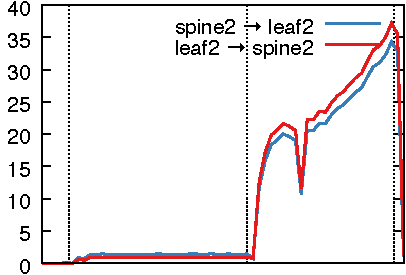
\includegraphics[width=.95\linewidth]{coll-prop-2-2816}
        \caption{At Port 0xb00 (spine2) \newline towards Port 0xa00 (leaf2)}%
        \label{fig:spine2-leaf2-prop}
    \end{subfigure}
    \begin{subfigure}{.45\linewidth}
        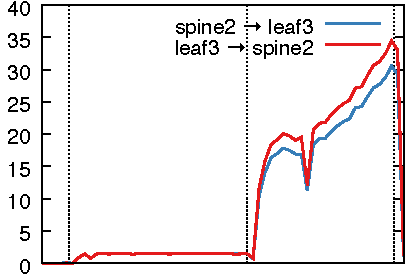
\includegraphics[width=.95\linewidth]{coll-prop-2-3072}
        \caption{At Port 0xc00 (spine2) \newline towards Port 0xa00 (leaf3)}%
        \label{fig:spine2-leaf3-prop}
    \end{subfigure}
    \begin{subfigure}{.45\linewidth}
        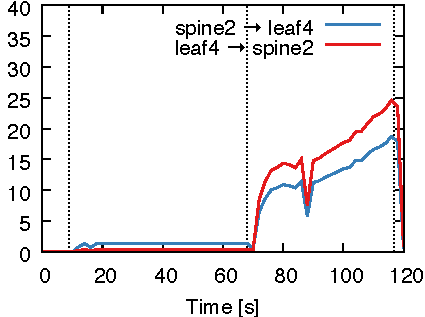
\includegraphics[width=.95\linewidth]{coll-prop-2-3328}
        \caption{At Port 0xd00 (spine2) \newline towards Port 0xa00 (leaf4)}%
        \label{fig:spine2-leaf4-prop}
    \end{subfigure}
    \caption{Throughput Measured at Ports on Switch spine2 (proposed)}%
    \label{fig:coll-spine2-prop}
\end{figure}


Figures~\ref{fig:coll-spine1-prop} and~\ref{fig:coll-spine2-prop} show
the change of throughput when using the proposed mechanism. In these
plots, the time of event occurrences recorded by the MPI application are
marked with vertical solid black lines. The time synchronization between
throughput change and event occurrences was made on the basis of the
timestamp. At \(t_1\) where MPI\_Bcast started, both RX and TX
throughput observed at the ports of spine1 rise steeply and then
maintain the amount of approximately 14Mbps and 9Mbps, respectively,
while there is no clear growth of throughput at the ports of spine2.
This indicates that only spine1 was utilized during the execution of
MPI\_Bcast. When MPI\_Bcast finished and then MPI\_Reduce started at
\(t_2\), a sharp fall of throughput at spine1 was observed, whereas a
rapid uptake in the throughput at spine2 was observed. After that, a
sharp drop of throughput at the ports of spine2 was observed immediately
when MPI\_Reduce finished (\(t_3\)). This measurement result indicates
that only spine2 was utilized during the execution of MPI\_Reduce. Based
on these observations, it is confirmed and verified that the network
control is synchronized with the execution of the MPI application.

\subsection{Evaluation of overhead}

\begin{figure}
    \centering
    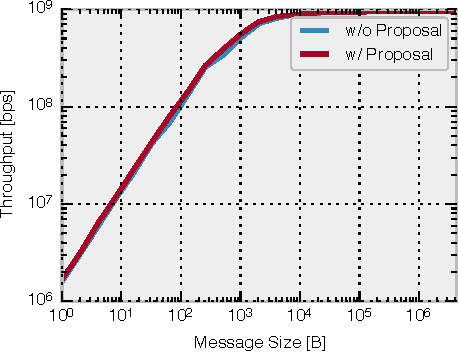
\includegraphics[width=0.6\linewidth]{overhead-bandwidth}
    \caption{Comparison of Bandwidth}%
    \label{fig:overhead-bandwidth}
\end{figure}

\begin{figure}
    \centering
    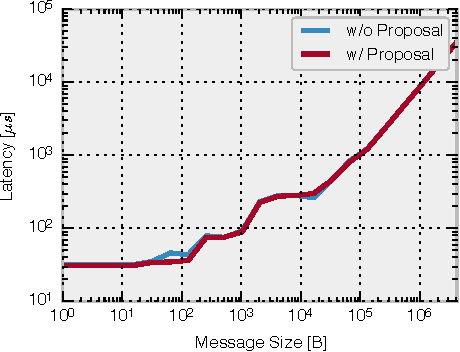
\includegraphics[width=0.6\linewidth]{overhead-latency}
    \caption{Comparison of Latency}%
    \label{fig:overhead-latency}
\end{figure}

\begin{figure}
    \centering
    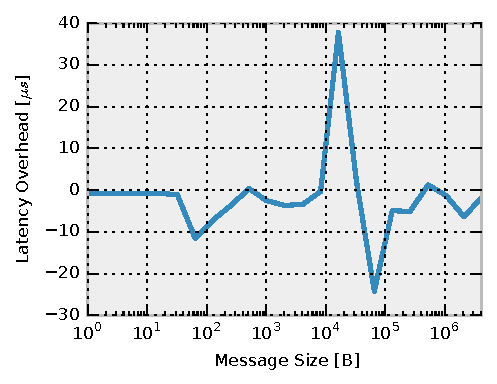
\includegraphics[width=0.6\linewidth]{overhead-latency2}
    \caption{Absolute Overhead to Latency}
    \label{fig:overhead-latency-2}
\end{figure}

The primary source of the overhead incurred by the proposed mechanism is
considered to be the tagging kernel module, because it requires
per-packet inspection and modification over all packets emitted from a
computing node. Additionally, rewriting the destination MAC address
header field in the switches to restore the true MAC address can also be
a source of overhead. In order to evaluate the total overhead caused by
the proposal, we measured the communication performance of
point-to-point MPI primitives using the OSU Micro-Benchmark Suite
5.3~\autocite{OhioStateUniversity2016} between node01 and node02 and
compared the result with and without the proposed mechanism. The reason
to measure the performance of point-to-point communication and not
collective communication is to remove unwanted influence from complex
algorithms and communication patterns of collective communications. The
osu\_bw benchmark and osu\_latency benchmark included in the OSU
Micro-Benchmark suite were used to measure the bandwidth and latency,
respectively.

Figure~\ref{fig:overhead-bandwidth} shows a comparison of the throughput
observed between node01 and node02. Fig.~\ref{fig:overhead-latency}
shows the comparison result of latency for the same computing node pair.
The plots in Fig.~\ref{fig:overhead-bandwidth} and
Fig.~\ref{fig:overhead-latency} represent the average of 500
measurements and 50,000 measurements, respectively.
Fig.~\ref{fig:overhead-latency-2} shows the overhead imposed to latency
by the proposed mechanism. These plots indicate that performance
degradation imposed by the proposed mechanism is practically negligible
for both bandwidth and latency.

In this experiment, we only evaluated the performance of point-to-point
primitives. However, the fact that collective primitives are often
implemented using multiple point-to-point
primitives~\autocites{Squyres2005}{mvapich} implies that the overhead
of the proposed mechanism is negligible for collective primitives as
well.

\section{Related Work}\label{sec:iv-related-work}

Several studies~\autocites{Mekky2014}{Cheng2014} have been carried out
to incorporate application-awareness into SDN\@. An extension to Open
vSwitch and OpenFlow has been proposed~\autocite{Mekky2014} to realize
an application-aware data plane. This extension adds flow tables with
application-specific actions to the packet processing pipeline of Open
vSwitch. Although this method covers most network applications, it is
not able to efficiently read and process the payload of a packet because
the flow matching mechanism has not been modified from the plain
OpenFlow design. Thus, only pre-defined header fields can be used as
matching criteria. Moreover, applying this method to bare-metal computer
clusters is challenging because the hardware switches were out of the
focus. The packet processing pipelines of commercial hardware switches
cannot be modified since they are implemented using unmodifiable
hardware. In contrast, our research supports existing hardware switches
and per-packet inspection.

An application-aware routing scheme for big data applications has been
presented in~\autocite{Cheng2014}. This routing scheme maintains a
global view of the network topology and link usage. Based on this global
view, the network controller dynamically allocates a path for each
Hadoop network flow so that congestion is avoided and network
utilization is increased. Experiments demonstrated that the
application-aware SDN routing significantly improved the speed of the
shuffle phase in Hadoop, in comparison with conventional routing
mechanisms such as ECMP and Spanning Tree. The concept of optimizing the
packet flow in the interconnect based on application-layer information
is similar to SDN-enhanced MPI\@. However, the scheme to synchronize flow
installation and a Hadoop job has not been clarified in this research.

Hybrid Flexibly Assignable Switch Topology (HFAST)~\autocite{Kamil2007}
interconnect architecture tailors the interconnect topology to meet the
communication requirements of different applications. This is achieved
by utilizing reconfigurable optical circuit switches to dynamically
provide the connection between packet switches. Additionally, a process
allocation algorithm optimized for HFAST architecture is also presented.
HFAST architecture can reduce required hardware resources compared to
conventional fat-tree interconnects. Our research is different from this
research in terms that a technical design to extract communication
patterns from applications and convey such information to the network
controller in real-time is exhibited.

A software-defined multicasting mechanism for MPI has been presented
in~\autocite{Arap2014}. This mechanism offloads collective MPI primitives to
programmable NICs and OpenFlow switches. This method heavily depends on
specialized hardware such as NetFPGA, whereas our proposal is software-based.

Multi-Protocol Label Switching~(MPLS) and UnisonFlow share the similar
idea of eliminating the need to examine packet payloads by encoding
upper layer information into fixed-length tags that are processable by
hardware. However, to the best of our knowledge, no work has tackled to
integrate MPI with label switching networks.

\section{Conclusion}\label{sec:iv-conclusion}

In this chapter, we have proposed UnisonFlow, a software-defined
coordination mechanism for SDN-enhanced MPI that performs network
control in synchronization with the execution of an application. The
proposed mechanism is characterized by a kernel-assisted approach to tag
packets that are emitted from computing nodes with the MPI context
information of each packet. Experiments conducted on a computer cluster
have verified the synchronization between network control and the
execution of the application. Moreover, evaluation experiments have
indicated that the overhead incurred by the coordination mechanism is
practically negligible.

There are still issues to be addressed in the future. First,
SDN-enhanced MPI primitives developed in our previous
work~\autocites{Dashdavaa2013}{Takahashi2014} need to be adjusted as MPI
primitive modules on the interconnect controller and tested to see if
they are accelerated compared to conventional MPI primitives. Second,
performance evaluation using real-world MPI applications is necessary.
Although we have developed some individual SDN-enhanced MPI primitives
and UnisonFlow as the coordination mechanism of message-passing
communication and computation, it is still unclear how these elements
can accelerate a practical application as a whole. Finally, we need to
investigate how this architecture can be adopted to a computer cluster
simultaneously running multiple jobs, which is common in practical
deployments. Since our current implementation of the UnisonFlow assumes
only one job running at the same time on a node, we need to enhance it
to support multiple concurrent jobs. This enhancement might involve an
integration with the job scheduler.
